\documentclass{article}
\usepackage[utf8]{inputenc}
\usepackage[right=.75in, left=1.5in, top=1.25in, bottom=1.25in]{geometry}
\usepackage{setspace}
\usepackage{fancyhdr}
\usepackage{imakeidx}
\usepackage{multirow}
\usepackage{tikz}
\usepackage{hyperref}
\hypersetup{
    colorlinks=true,
    linkcolor=black,
    filecolor=magenta,      
    urlcolor=cyan,
    pdftitle={Overleaf Example},
    pdfpagemode=FullScreen,
    }
    
    \title{UNIVERSIDAD NACIONAL DE SAN AGUSTÍN\\
MAESTRÍA EN CIENCIAS DE LA COMPUTACIÓN\\
Algoritmos y Estructura de datos\\Práctica 4}
\author{Christian Néstor Barriga Marcapura\\
        Weimar Ccapatinta Huamani\\ Roger Gutierrez Espinoza}
\date{Setiembre 12, 2022}


\begin{document}

\maketitle

\tableofcontents
\newpage
\pagestyle{fancy}
\fancyhf{}
\lhead{Algoritmos y Estructura de datos}
\rhead{Práctica 4}
\chead{UNSA}
\rfoot{\thepage}{}
\section{Introducción}
\doublespacing En ciencias de la computación, es una estructura de datos de particionado del espacio que organiza los puntos en un Espacio euclídeo de k dimensiones. Los árboles kd son un caso especial de los árboles BSP.

Un árbol kd emplea sólo planos perpendiculares a uno de los ejes del sistema de coordenadas. Esto difiere de los árboles BSP, donde los planos pueden ser arbitrarios. Además, todos los nodos de un árbol kd, desde el nodo raíz hasta los nodos hoja, almacenan un punto. Mientras tanto, en los árboles BSP son las hojas los únicos nodos que contienen puntos (u otras primitivas geométricas). Como consecuencia, cada plano debe pasar a través de uno de los puntos del árbol kd.

\section{Ejercicios}
\doublespacing 
\subsection{Funciones: build-kdtree, getHeight, generate-dot}
Se realizó la implementación del algoritmo considerando las funciones mencioandas, tal como se muestra en la figura 1.
 \center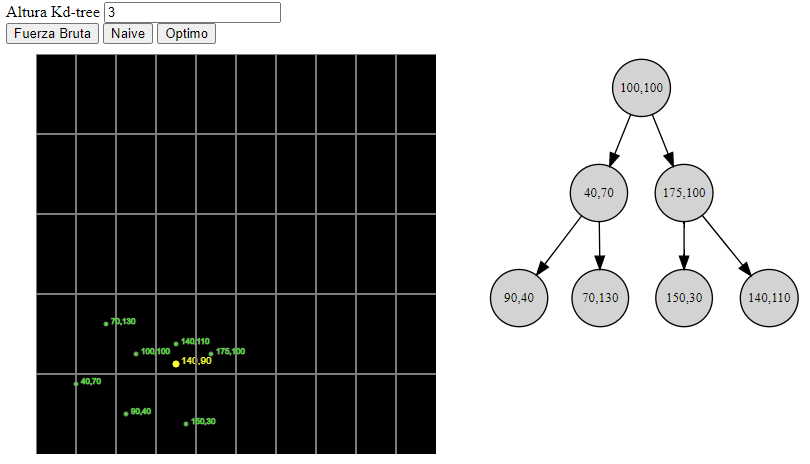
\includegraphics[trim={0.cm 0.cm 0cm 0.cm},clip,scale=0.7]{Practica 4/pregunta2.png}
 \center Figura 1 Funciones Kd Tree - Elaboración propia
 
\newpage\
 
 \begin{flushleft}
Se implementarion tres funcionalidades, Fuerza bruta, Naive y optimo.\\
La fuerza bruta saca la distancia entre dos puntos y obtiene el menor.\\
\end{flushleft}
 \center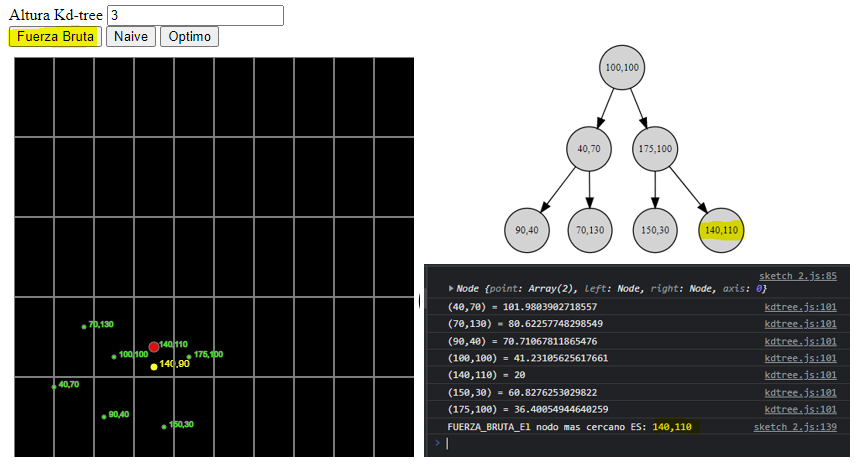
\includegraphics[trim={0.cm 0.cm 0cm 0.cm},clip,scale=0.7]{Practica 4/Fbruta.png}
 \center Figura 2 Fuerza bruta - Elaboración propia
 \begin{flushleft}
Naive, sigue a los nodos comparando con los ejes, cuando estan cerca del límite, no revisa el otro nodo y tiende a equivocarse\\
\end{flushleft}
 \center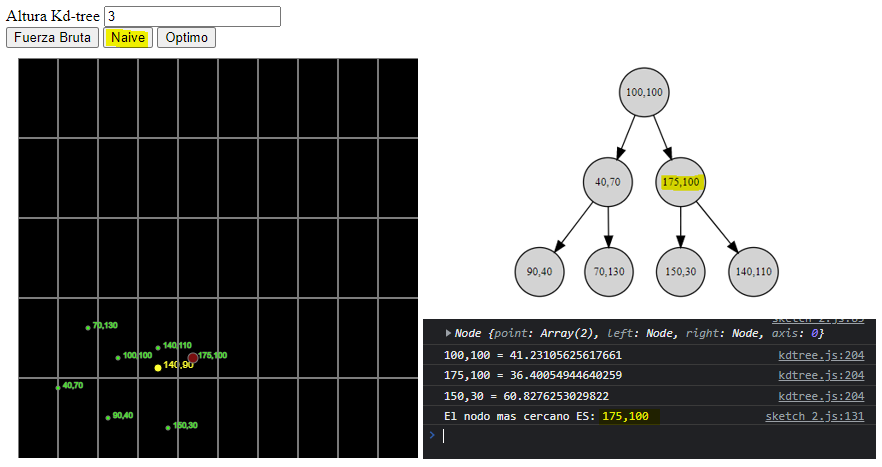
\includegraphics[trim={0.cm 0.cm 0cm 0.cm},clip,scale=0.7]{Practica 4/naive.png}
 \center Figura 3 Función naive  - Elaboración propia
 \begin{flushleft}
Y finalmente Optimo\\
\end{flushleft}
 \center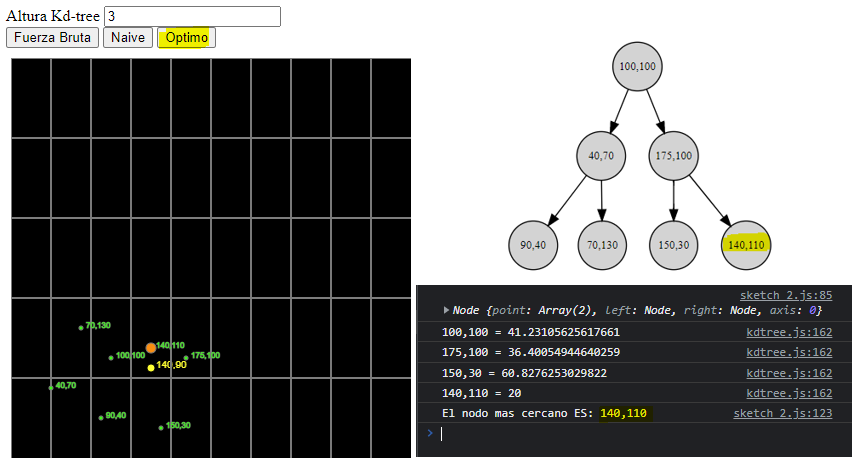
\includegraphics[trim={0.cm 0.cm 0cm 0.cm},clip,scale=0.7]{Practica 4/Optimo.png}
 \center Figura 4 Busqueda óptima - Elaboración propia
\newpage\
\begin{flushleft}
\subsection{Implementación de closest point}
En la siguiente figura se muestra coomo esta implementado el Closest point.
\end{flushleft}
 \center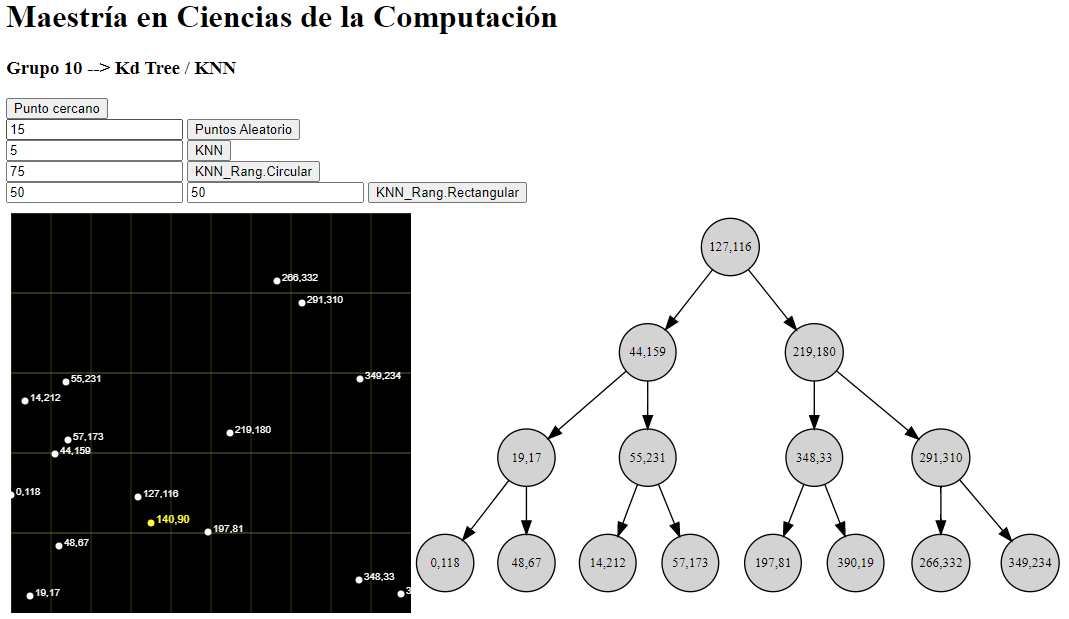
\includegraphics[trim={0.cm 0.cm 0cm 0.cm},clip,scale=0.6]{Practica 4/pregunta 7.png}
 \center Figura 5 Closest point - Elaboración propia
\begin{flushleft}
\subsection{Función KNN}
\end{flushleft} 
 \center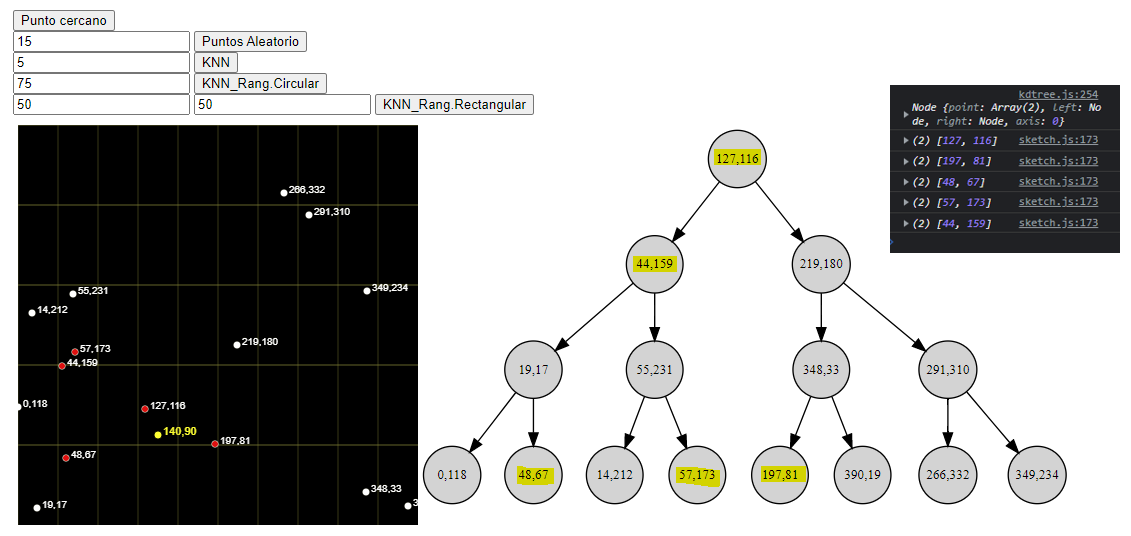
\includegraphics[trim={0.cm 0.cm 0cm 0.cm},clip,scale=0.5]{Practica 4/knn.png}
 \center Figura 6 Función KNN - Elaboración propia.\\
 \begin{flushleft}
 Se consideraron dos tipos de range query:\\
 Del tipo circular\\
 \end{flushleft} 
 \center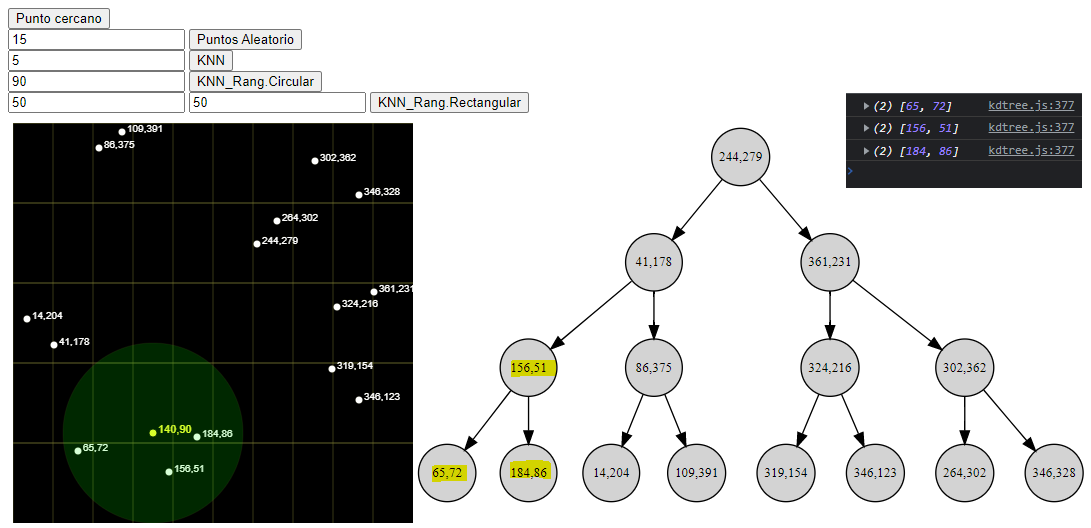
\includegraphics[trim={0.cm 0.cm 0cm 0.cm},clip,scale=0.5]{Practica 4/circular.png}
 \center Figura 7 Función KNN query circular - Elaboración propia\\
 \begin{flushleft}
 Del tipo rectangular, realizando el sombreado del área que abarca cada figura.\\
 \end{flushleft} 
  \center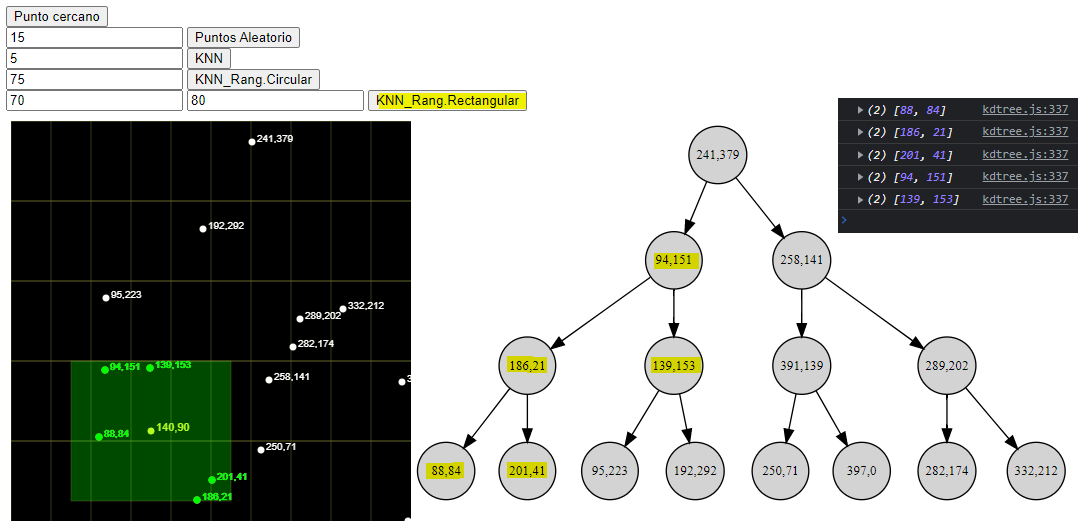
\includegraphics[trim={0.cm 0.cm 0cm 0.cm},clip,scale=0.5]{Practica 4/rectagular.png}
 \center Figura 8 Función KNN query rectangular- Elaboración propia
 \begin{flushleft}
\section{Implementación}
Se envía el siguiente enlace en Github, donde se encuentran los codigos elaborados y con las animaciones respectivas.\\
\url{https://github.com/weicap/Practica-4}
 \end{flushleft} 
\end{document}